\documentclass[tikz,border=4pt]{standalone}
\usetikzlibrary{positioning}

\begin{document}
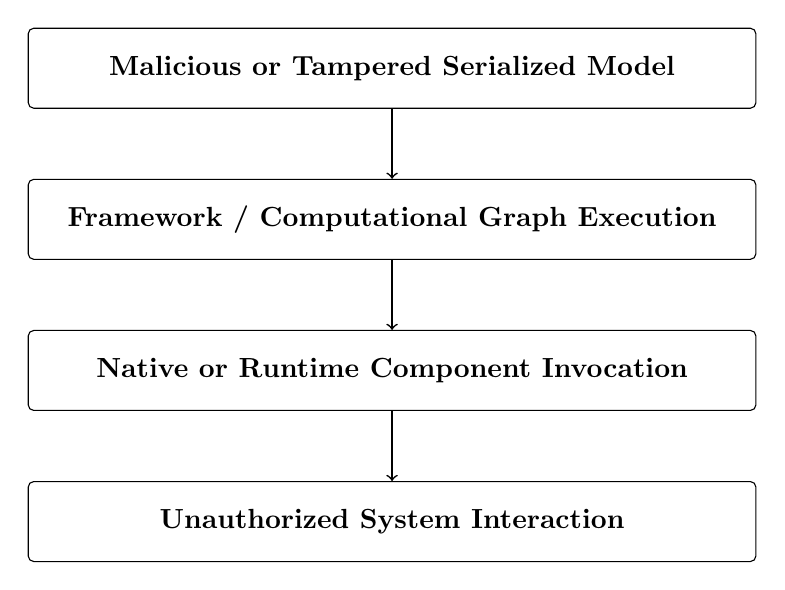
\begin{tikzpicture}[
  stage/.style={
    draw,
    rounded corners=2pt,
    text width=3.5in,
    minimum height=0.4in,
    align=center,
    font=\bfseries,
    inner sep=5pt
  },
  node distance=0.35in
]
\node[stage] (model) {Malicious or Tampered Serialized Model};
\node[stage, below=of model] (graph) {Framework / Computational Graph Execution};
\node[stage, below=of graph] (runtime) {Native or Runtime Component Invocation};
\node[stage, below=of runtime] (impact) {Unauthorized System Interaction};

\draw[->, semithick] (model) -- (graph);
\draw[->, semithick] (graph) -- (runtime);
\draw[->, semithick] (runtime) -- (impact);
\end{tikzpicture}
\end{document}
